\documentclass[twocolumn]{article}
\usepackage{graphicx}
\usepackage{fullpage}
\title{A brief description of exponential function and implementation in C}
\author{P. A. Samu}
\date{}
\begin{document}
\maketitle

\begin{abstract}
We shall introduce the exponential function and then implement it in the C programming language. In the end we shall compare the implementation with the exponential function already implemented in the math header file.
\end{abstract}

\section{Exponential function}
The exponential function, $\exp(x)$, can be defined in many ways. One of the ways is defining it by the following limit:

\begin{equation}
	\exp(x)=\lim_{n \rightarrow \infty}(1+\frac{x}{n})^n
\end{equation}
Another important characteristic of the exponential function, which also distinguishes it from every other function, is that the derivative is equal to itself.
\begin{equation}
	\frac{d}{dx}\exp(x)=\exp(x)
\end{equation}

\section{Implementation}
The way we have implemented the exponential function in C language, is to consider its power series expansion first and foremost.
\begin{equation}
	\exp(x)=\sum_{n=0}^{\infty} 
\end{equation}
The way to implement this power series is to take a number of terms. More terms lead to more precision, but also longer compilation times. In this implementation we take the first eleven terms (so up to $n=10$). Instead of writing it like this, we write the expansion in the following way.

\begin{equation}
	\exp(x)=1+x(1+\frac{x}{2}(1+\frac{x}{3}))
\end{equation}
This is just the first four terms, in the implementation we continue until we have ten terms. This way we get multiplication instead of powers, which is faster. 

\section{Plots}
Here is a plot of the implementation of the exponential function in the C programming language. We plot it versus the built-in exponential function from the math.h headerfile. 

\begin{figure}[h]
	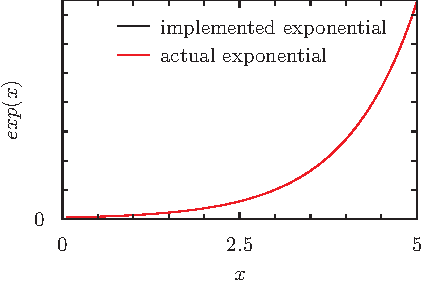
\includegraphics{fig-pyxplot.pdf}
	\caption{Plot of exponential function implementation via pyxplot "pdf" terminal.}
	\label{fig:expimp}
\end{figure}
We see that the graphs lay directly on top of eachother, which means our implementation works as intended. 

\end{document}

